\documentclass{beamer}
\setbeamertemplate{navigation symbols}{}
\usetheme{}
\usepackage[english]{babel}
\setbeamercovered{transparent}
\usepackage{times}
\usepackage[T1]{fontenc}
\usepackage{beamerthemeshadow}
\begin{document}
\title[Sreekrishnapuram]{Will NoSQL Database Live Up to Their Promises?}
\subtitle{Neal Leavitt  , \ IEEE,2010}
\author[Govt. Engineering College]{}
\date{\today} 

\begin{frame}
\titlepage
\end{frame}

\begin{frame}
\\
\medskip 
Group Members:\\
\hspace*{3.5cm}Sajmiya S \hspace*{2.25cm}(EPAKECS042)
\\\hspace*{3.5cm}Sahya Satheesan \hspace*{1.5cm}(EPAKECS041)
\\\hspace*{3.5cm}Rosni K V \hspace*{2.35cm}(EPAKECS040)
\end{frame}

\begin{frame}\frametitle{Table of contents}\tableofcontents
\end{frame}

\section[]{Introduction }
\begin{frame}\frametitle{Introduction}
\begin{center}
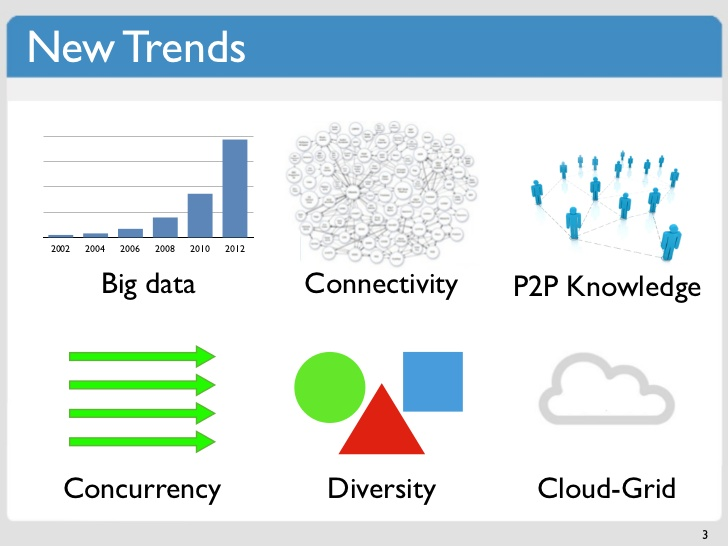
\includegraphics[scale=.35]{slide-8-728.jpg}
\end{center}
\end{frame}
\begin{frame}\frametitle{Introduction}
\begin{itemize}
\begin{center}
\textbf{Organizations that collect large amounts of unstructured data are increasingly turning to nonrelational databases, now frequently called NoSQL databases}
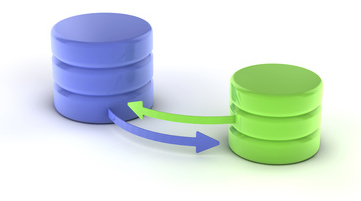
\includegraphics{Fotolia_20338317_XS2.jpg}
\end{itemize}
\end{center}
\end{frame}
\begin{frame}\frametitle{Introduction}
\begin{center}

\includegraphics{nosqlr.png}
\end{center}
\end{frame}
\begin{frame}\frametitle{Introduction}
\begin{itemize}
\begin{center}
\textbf{Includes-hierarchical,graph and object oriented databases. \newline \newline Different NoSQL db takes different approaches. \newline\newline  Handle unstructured data such as word-processing files, e-mail, multimedia, and social media efficiently.\newline\newline Enables better performance-important for applications with large amount of data.\newline\newline Amazon and Google developed Dynamo and BigTable nosql db resp. }
\end{center}
\end{itemize}
\end{frame}

\subsection[]{In the Beginning}
%\subsection[]{}
\begin{frame}\frametitle{In the Beginning}
\vspace{0.5cm}
\begin{itemize}
\item Late Edgar Codd,a former IBM fellow,is generally credited with creating the relational-database model in 1970.\vspace{0.5cm}
\item A RDB is a set of tables containing data fitted into predefined categories.\vspace{0.5cm}  
\item Table with rows and columns -can access or reassemble the data in different ways(w/o having to reorganize the db tables).
\\
\end{itemize}
\end{frame}
\begin{frame}\frametitle{In the Beginning}
\item RDB work best with structured data.\vspace{0.5cm}
\item Not the case with unstructured data,such as that found in word-processing documents and images.\vspace{0.5cm}
\end{frame}


\subsection[]{Relational DB Limitations}
\begin{frame}\frametitle{Relational DB Limitations}
\begin{itemize}\vspace{0.5cm}
\item Structure of data is predefined by the layout of tables and fixed names and types of columns.
\newline
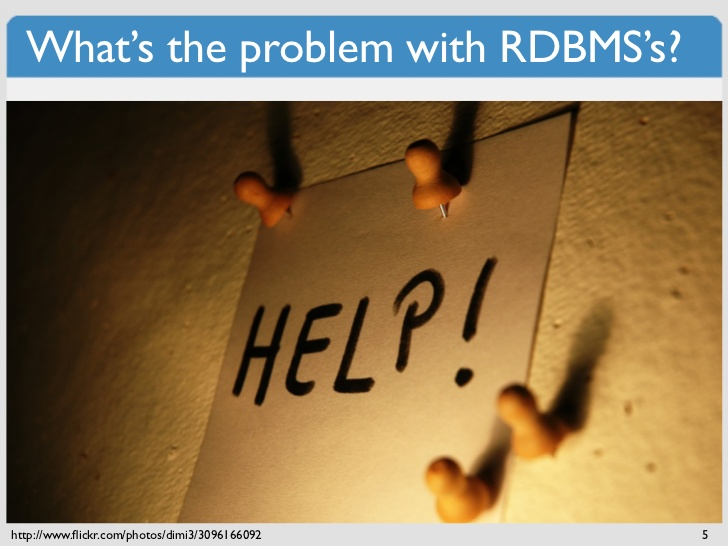
\includegraphics[scale=.30]{slide-12-728.jpg}
\end{itemize}
\end{frame}
\begin{frame}\frametitle{Relational DB Limitations}
\begin{itemize}\vspace{.5 cm}
\begin{center}
\textbf{ Limitations}
\end{center}
\item Scaling
\item Complexity
\item SQL
\item Large feature set\newline
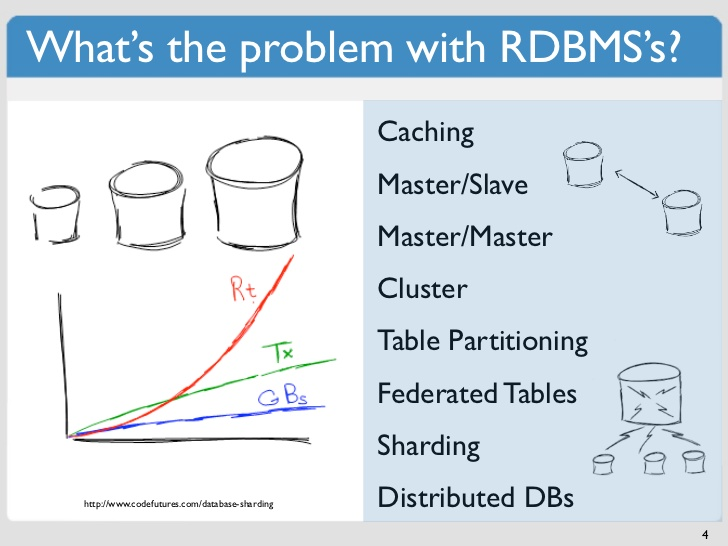
\includegraphics[scale=.25]{slide-10-728.jpg}
\end{itemize}
\end{frame}

\section[]{Inside NoSQL DataBases}
\begin{frame}\frametitle{Inside NoSQL DataBases}
\begin{itemize}
\item Limitations of relational databases  , vendors and users are increasingly turning to NoSQL databases.
\newline
\item Amazon was one of the first major companies to store much of its important corporate data in a non-relational database.
\newline
\end{itemize}
\end{frame}
\subsection[]{The Technology}
\begin{frame}\frametitle{The Technology}
\textbf{There are three popular types of NoSQL databases}
\begin{itemize}
\item Key-value stores
\item Column-oriented databases
\item Document-based stores.
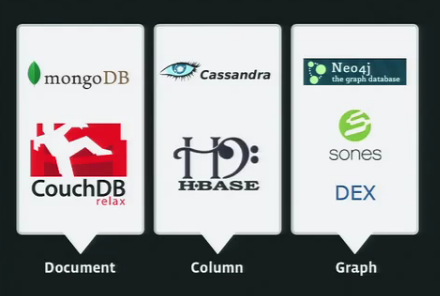
\includegraphics[scale=0.55]{nosql.png}
\end{itemize}
\end{frame}

\begin{frame}\frametitle{The Technology}
\textbf{Key-value stores}
\begin{itemize}
\item A key-value store is a system that stores values indexed for retrieval by keys.
\item Can hold structured or unstructured data.
\item Amazon’s SimpleDB is a Web service that provides core database functions of information indexing and querying in the cloud.
\end{itemize}
\end{frame}

\begin{frame}\frametitle{The Technology}
\textbf{Column-oriented databases}
\begin{itemize}
\item Contain one extendable column of closely related data.
\item Facebook-Cassandra to help power its website
\item Apache Software Foundation developed Hbase
\end{itemize}
\end{frame}

\begin{frame}\frametitle{The Technology}
\textbf{Document-based stores}
\begin{itemize}
\item Store and organize data as collections of documents.
\item Apache Software Foundation- CouchDB as an open source.
\item Basho Technologies’ Riak-  open source database suitable for Web-based applications.
\end{itemize}
\end{frame}

\subsection[]{Open Source}
\begin{frame}\frametitle{Open Source}
\textbf{Most NoSQL db are open source,reflecting developments in the overall software market}
\newline\newline
\textbf{Do better in os environment,which lets users perform technical evaluations at low cost.}
\end{frame}

\section[]{NoSQL PROS & CONS}
\subsection[]{Advantages}
\begin{frame}\frametitle{NoSQL PROS & CONS}
\textbf{Advantages}
\begin{itemize}
\item Generally process data faster than relational databases.
\item Developers usually don’t have their NoSQL databases support ACID, in order to increase performance.\newline ACID (atomicity,consistency, isolation, durability)
\item NoSQL databases are also often faster.
\end{itemize}
\end{frame}
\begin{frame}\newline
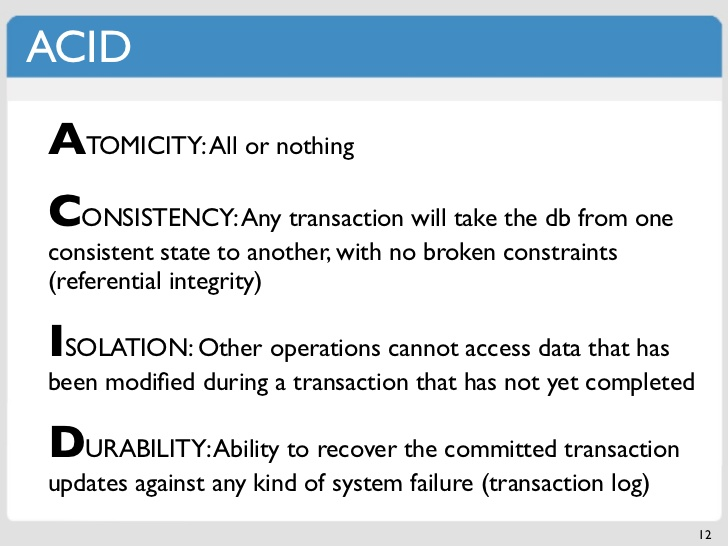
\includegraphics[scale=.45]{slide-20-728.jpg}
\end{frame}

\subsection[]{Disadvantages}
\begin{frame}\frametitle{NoSQL PROS & CONS}
\textbf{Dis-advantages}
\begin{itemize}
\item NoSQL databases usually do not support ACID, but this can cause problems when used for applications that require great precision.
\end{itemize}
\end{frame}
\section[]{Concerns and Doubts}
\begin{frame}\frametitle{Concerns and Doubts}
\textbf{NoSQL database faces several challenges..}\newline\newline
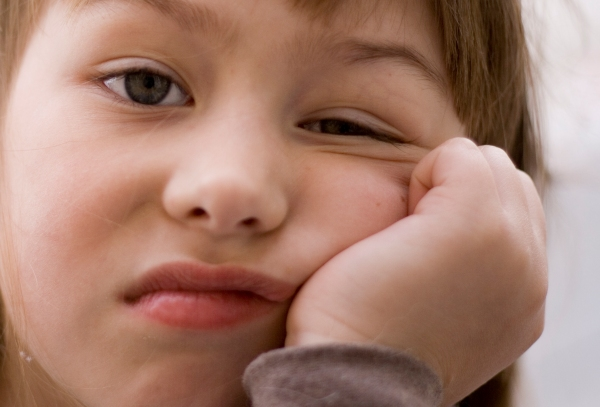
\includegraphics[scale=1]{bored-girl.jpg}
\end{frame}
\begin{frame}\frametitle{Concerns and Doubts}
\vspace{0.5cm}
\begin{itemize}
\item Overhead and Complexity
\newline 
\textit{Don't work with SQL \newline Require manual query programming which can be fast for simple tasks but time consuming for others.\newline In addition,complex query programming for the databases can be difficult.}
\newline
\item Reliability \newline
\textit{ Don't support ACID,so they don't natively offer the degree of reliability that ACID provides,that is to apply they must perform additional programming}
\newline \vspace{0.5cm}
\end{itemize}
\end{frame}

\begin{frame}\frametitle{Concerns and Doubts}
\begin{itemize}
\item Consistency \newline
\textit{Because NoSQL db don't natively support ACID transaction,they also could compromise consistency,unless manual support is provided.\newline Not providing consistency enables better performance and scalability but is a problem for certain types of applications and transaction,such as those involved in banking.}
\newline
\item Unfamiliarity with the technology \newline
\textit{Most organisations are unfamiliar with Nosql db\newline May not feel knowledgeable enough to choose one or even to determine that the approach might be better for their purposes.}
\end{itemize}
\end{frame}

\begin{frame}\frametitle{Concerns and Doubts}
\begin{itemize}
\item Limited Eco-structure \newline
\textit{Unlike commercial relational databases,many open source Nosql apps don't yet come with customer support in management tools.} \newline
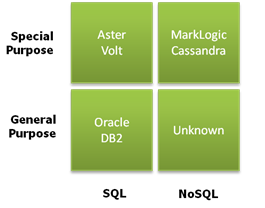
\includegraphics[scale=.60]{nosql-quadrant11.png}
\end{itemize}
\end{frame}

\subsection[]{Conclusion}
\begin{frame}\frametitle{Conclusion}
\begin{center}
\textbf{During the next 5 years,according to RedMonk's O'Grady,NoSQL proponents will focus on developing better application compatibility and management tools}
\newline\newline
\textbf{According to Dave Rosenberg,Nosql databases will be used largely for working with unstructured data in ways that require scalability}
\newline\newline
\textbf{Nosql adoption will be small-scale and only in small niches because relational databases are more mature and represent huge investments by vendors and users,said Anant Jhingran}
\end{center}
\end{frame}

\begin{frame}\frametitle{Conclusion}
\begin{center}
\textbf{During the next one or two years,O'Grady predicted,users will adopt NoSQL db primarily for specialized projects,such as those that are distributed,that involve large amounts of data,or that must scale.}
\newline\newline
\textbf{NoSQL databases won't replace relational databases,but instead will become a better option for certain types of projects.}
\newline\newline
\textbf{There will be a growing realization that the relational database in use today are often good tools but that other tools have their place as well}
\end{center}
\end{frame}

\begin{frame}\frametitle{Thank You!!!}
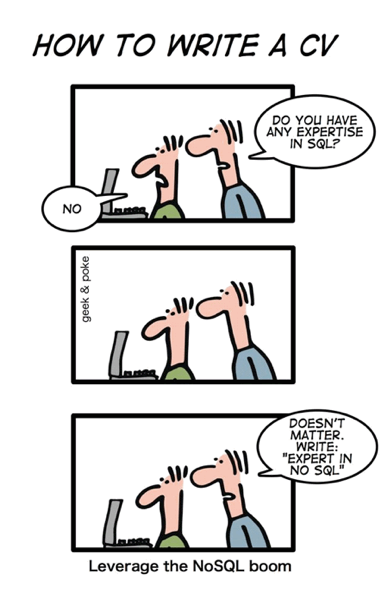
\includegraphics[scale=.35]{nosql-expert.png}
\end{frame}

\end{document}